\documentclass[runningheads]{llncs}

\usepackage[T1]{fontenc}
\usepackage[utf8]{inputenc}
\usepackage{amsmath,amssymb,amsfonts}
\usepackage{booktabs,tabularx,array}
\usepackage{graphicx}
\usepackage{hyperref}
\hypersetup{hidelinks,
  pdftitle={Context-Dependent Selection of Established Urban Routing Policies:
            Regime Effects, Decision Value, and Generalization Limits},
  pdfauthor={Anonymous Author(s)},
  pdfsubject={Routing-policy selection; algorithm selection; decision regret},
  pdfkeywords={routing-policy selection, algorithm selection, decision regret,
               microsimulation, distribution shift, selective prediction}}

\newcommand{\CO}{CO\textsubscript{2}}
\graphicspath{{figures/}}
\renewcommand{\tabularxcolumn}[1]{m{#1}}


\begin{document}

\title{Context-Dependent Selection of Established Urban Routing Policies:
Regime Effects, Decision Value, and Generalization Limits}
\titlerunning{Context-Dependent Selection of Urban Routing Policies}
\author{Anonymous Author(s)}
\authorrunning{Anonymous Author(s)}
\institute{Anonymous institution(s)}
\maketitle

% GENERATED by analysis/emit_numbers.py -- do not edit.
% Every numeric claim in the manuscript resolves through a macro here.
\newcommand{\NumAbstainRate}{61\%}
\newcommand{\NumBFiveCVaR}{2.6}
\newcommand{\NumBFiveExact}{39\%}
\newcommand{\NumBFiveGapClosed}{1.1\%}
\newcommand{\NumBFiveMax}{6.1}
\newcommand{\NumBFiveMedian}{0.07}
\newcommand{\NumBFiveRegret}{0.42}
\newcommand{\NumBFiveTopOne}{33\%}
\newcommand{\NumBFiveWithinNoise}{98\%}
\newcommand{\NumBFourBeatsBOne}{yes}
\newcommand{\NumBFourCVaR}{2.5}
\newcommand{\NumBFourExact}{66\%}
\newcommand{\NumBFourGapClosed}{24.7\%}
\newcommand{\NumBFourMax}{6.9}
\newcommand{\NumBFourMedian}{0.00}
\newcommand{\NumBFourRegret}{0.32}
\newcommand{\NumBFourTopOne}{58\%}
\newcommand{\NumBFourVsBOne}{-0.17}
\newcommand{\NumBFourWithinNoise}{93\%}
\newcommand{\NumBOneCVaR}{3.5}
\newcommand{\NumBOneExact}{62\%}
\newcommand{\NumBOneGapClosed}{-15.1\%}
\newcommand{\NumBOneMax}{6.6}
\newcommand{\NumBOneMedian}{0.00}
\newcommand{\NumBOneRegret}{0.49}
\newcommand{\NumBOneTopOne}{54\%}
\newcommand{\NumBOneWithinNoise}{95\%}
\newcommand{\NumBThreeCVaR}{1.0}
\newcommand{\NumBThreeExact}{69\%}
\newcommand{\NumBThreeGapClosed}{67.6\%}
\newcommand{\NumBThreeMax}{2.1}
\newcommand{\NumBThreeMedian}{0.00}
\newcommand{\NumBThreeRegret}{0.14}
\newcommand{\NumBThreeTopOne}{69\%}
\newcommand{\NumBThreeWithinNoise}{100\%}
\newcommand{\NumBTwoCVaR}{4.3}
\newcommand{\NumBTwoExact}{49\%}
\newcommand{\NumBTwoGapClosed}{-63.8\%}
\newcommand{\NumBTwoMax}{8.0}
\newcommand{\NumBTwoMedian}{0.02}
\newcommand{\NumBTwoRegret}{0.69}
\newcommand{\NumBTwoTopOne}{41\%}
\newcommand{\NumBTwoWithinNoise}{93\%}
\newcommand{\NumBZeroCVaR}{2.6}
\newcommand{\NumBZeroExact}{37\%}
\newcommand{\NumBZeroMax}{6.1}
\newcommand{\NumBZeroMedian}{0.08}
\newcommand{\NumBZeroRegret}{0.42}
\newcommand{\NumBZeroTopOne}{31\%}
\newcommand{\NumBZeroWithinNoise}{98\%}
\newcommand{\NumBestCOTwoDiffers}{59}
\newcommand{\NumBestCOTwoDiffersPct}{42\%}
\newcommand{\NumBestCThreeDiffers}{61}
\newcommand{\NumBestCThreeDiffersPct}{43\%}
\newcommand{\NumCapBypass}{1500}
\newcommand{\NumConstantRule}{31.7\%}
\newcommand{\NumContexts}{143}
\newcommand{\NumContextsAnalysed}{142}
\newcommand{\NumCorrC1C2}{+0.9645}
\newcommand{\NumCorrC1C3}{+0.9618}
\newcommand{\NumCorrC2C3}{+0.8758}
\newcommand{\NumCostSBS}{312.2}
\newcommand{\NumCostVBS}{311.7}
\newcommand{\NumGOneNPolicies}{3}
\newcommand{\NumGOnePolicies}{P1, P3, P4}
\newcommand{\NumGOneResMax}{1.8\%}
\newcommand{\NumGOneResMedian}{0.28\%}
\newcommand{\NumGOneUnresMedian}{0.04\%}
\newcommand{\NumGOneUnresolved}{126}
\newcommand{\NumGOneUnresolvedPct}{88.7\%}
\newcommand{\NumGOneVerdict}{passes}
\newcommand{\NumGapP1P2}{+46.28}
\newcommand{\NumGapP1P3}{+46.65}
\newcommand{\NumGapP1P4}{+46.45}
\newcommand{\NumGapP2P3}{+0.38}
\newcommand{\NumGapP2P4}{+0.17}
\newcommand{\NumGapP3P4}{-0.21}
\newcommand{\NumGlobalSBS}{P3}
\newcommand{\NumHeadroom}{0.42}
\newcommand{\NumHeadroomMax}{6.1}
\newcommand{\NumHeadroomPct}{0.14\%}
\newcommand{\NumIdentP1P2}{0\%}
\newcommand{\NumIdentP1P3}{0\%}
\newcommand{\NumIdentP1P4}{0\%}
\newcommand{\NumIdentP2P3}{45\%}
\newcommand{\NumIdentP2P4}{50\%}
\newcommand{\NumIdentP3P4}{38\%}
\newcommand{\NumInvalidContexts}{0}
\newcommand{\NumInvalidRuns}{0}
\newcommand{\NumMeanCompletion}{1.0000}
\newcommand{\NumMeanIdentity}{22.2\%}
\newcommand{\NumMinCompletion}{1.000}
\newcommand{\NumOODFivePenAbstain}{54\%}
\newcommand{\NumOODFivePenBFive}{1.56}
\newcommand{\NumOODFivePenBFour}{0.38}
\newcommand{\NumOODFivePenBOne}{1.01}
\newcommand{\NumOODFivePenBZero}{1.56}
\newcommand{\NumOODFivePenN}{46}
\newcommand{\NumOODFivePenSupport}{100\%}
\newcommand{\NumOODFourLagAbstain}{63\%}
\newcommand{\NumOODFourLagBFive}{0.49}
\newcommand{\NumOODFourLagBFour}{0.69}
\newcommand{\NumOODFourLagBOne}{0.42}
\newcommand{\NumOODFourLagBZero}{0.49}
\newcommand{\NumOODFourLagN}{46}
\newcommand{\NumOODFourLagSupport}{100\%}
\newcommand{\NumOODSevenIncAbstain}{64\%}
\newcommand{\NumOODSevenIncBFive}{0.21}
\newcommand{\NumOODSevenIncBFour}{5.57}
\newcommand{\NumOODSevenIncBOne}{1.62}
\newcommand{\NumOODSevenIncBZero}{0.21}
\newcommand{\NumOODSevenIncN}{70}
\newcommand{\NumOODSevenIncSupport}{0\%}
\newcommand{\NumOODSixGreenAbstain}{86\%}
\newcommand{\NumOODSixGreenBFive}{0.95}
\newcommand{\NumOODSixGreenBFour}{0.68}
\newcommand{\NumOODSixGreenBOne}{1.67}
\newcommand{\NumOODSixGreenBZero}{0.95}
\newcommand{\NumOODSixGreenN}{36}
\newcommand{\NumOODSixGreenSupport}{100\%}
\newcommand{\NumOODTwoLowAbstain}{0\%}
\newcommand{\NumOODTwoLowBFive}{0.53}
\newcommand{\NumOODTwoLowBFour}{0.53}
\newcommand{\NumOODTwoLowBOne}{0.63}
\newcommand{\NumOODTwoLowBZero}{0.53}
\newcommand{\NumOODTwoLowN}{108}
\newcommand{\NumOODTwoLowSupport}{100\%}
\newcommand{\NumOutOfSupportRate}{5\%}
\newcommand{\NumParetoNonSingleton}{88.7\%}
\newcommand{\NumParetoP1}{14}
\newcommand{\NumParetoP2}{74}
\newcommand{\NumParetoP3}{114}
\newcommand{\NumParetoP4}{133}
\newcommand{\NumParetoPctP1}{10\%}
\newcommand{\NumParetoPctP2}{52\%}
\newcommand{\NumParetoPctP3}{80\%}
\newcommand{\NumParetoPctP4}{94\%}
\newcommand{\NumPolicies}{4}
\newcommand{\NumRuns}{2{,}853}
\newcommand{\NumSBSOptimalPct}{31\%}
\newcommand{\NumSameOrderC1C2}{46\%}
\newcommand{\NumSameOrderC1C3}{46\%}
\newcommand{\NumSameOrderC2C3}{25\%}
\newcommand{\NumSatArterial}{1761}
\newcommand{\NumSatNorth}{1596}
\newcommand{\NumSatSpread}{1.8\%}
\newcommand{\NumSeeds}{5}
\newcommand{\NumStumpBest}{50.7\%}
\newcommand{\NumStumpBestFactor}{gc}
\newcommand{\NumStumpTwo}{60.6\%}
\newcommand{\NumTeleports}{0}
\newcommand{\NumTwoPathRatio}{1.97}
\newcommand{\NumWinAllP1}{14}
\newcommand{\NumWinAllP2}{42}
\newcommand{\NumWinAllP3}{41}
\newcommand{\NumWinAllP4}{45}
\newcommand{\NumWinResP1}{6}
\newcommand{\NumWinResP2}{0}
\newcommand{\NumWinResP3}{5}
\newcommand{\NumWinResP4}{5}

\begin{abstract}
Navigation systems implement established routing objectives --- shortest
distance, reactive travel time, capacity-aware load balancing,
reliability-aware routing --- but commit to one by design rather than by traffic
condition. We ask whether that commitment should be made per context, and
separate two questions usually merged: whether the preferred policy varies with
conditions, and whether exploiting that variation is worth anything.

In \NumRunsMain{} microsimulation runs over \NumContexts{} contexts
(\NumSeeds{} paired seeds per policy) spanning demand, signal timing,
penetration, information lag, disruption and alternative capacity, the
preference does vary: three of four policies are strictly best somewhere by a
seed-resolved margin, and \NumParetoNonSingleton{} of contexts have a
non-singleton Pareto set over journey time, \CO{} and stopped delay --- with the
reliability-aware policy minimising stopped delay in \NumSpecCThreePct{} of
contexts while rarely minimising journey time. Exploiting it is nevertheless
worth \NumHeadroom\,s per vehicle, \NumHeadroomPct{} of the single-best fixed
policy's mean journey time, because that policy's average gain where it wins is
\NumAsymRatio$\times$ its average loss where it does not; selecting the wrong
fixed policy costs \NumFixedPenPctAbsPOne{} of the same baseline.

Within that margin, a selector predicting the winner's identity is \emph{more
accurate and more costly} than the fixed policy, whereas one predicting each
policy's \emph{advantage} closes \NumBFourGapClosed{} of the available gap.
Across \NumOODNTotal{} shift splits the unguarded selector helps on
\NumOODNHelps{}, is indistinguishable on \NumOODNNeutral{} and harms on
\NumOODNHarms{}; a support-and-confidence gate recovered the fixed policy
exactly on every harmful split, at the cost of the in-distribution gain, and one
split shows a shift the gate cannot see because it leaves the feature space
unchanged. The benchmark separates three questions usually treated as one:
complementarity, decision value, and deployability. We introduce no routing,
learning or multi-criteria decision algorithm.

\keywords{Routing-policy selection \and Algorithm selection \and Decision
regret \and Microsimulation \and Distribution shift \and Selective prediction.}
\end{abstract}


\section{Introduction}

A guidance system makes two decisions, not one.

\begin{description}
\item[Level 1.] Which routing \emph{policy} should be active under the current
traffic conditions?
\item[Level 2.] Given that policy, which route does each guided vehicle
receive?
\end{description}

Level 2 is the subject of a large literature. This paper concerns Level 1, and
treats the policies themselves as fixed, published objectives.

The question matters because established policies embody different assumptions.
Distance minimisation assumes the shortest corridor can absorb what is sent to
it. Reactive travel-time routing assumes recent measurements predict the near
future, which fails when a large guided cohort acts on them
simultaneously~\cite{arnott1991information,acemoglu2018braess}. Load balancing
assumes capacity is unevenly distributed and worth equalising. Reliability-aware
routing assumes travel-time variability is itself a cost. Each assumption holds
in some conditions and not others, so the policy that should be active plausibly
depends on the traffic --- and production systems nevertheless fix it at design
time.

\paragraph{The gap this paper addresses.}
Showing that the preferred policy changes with conditions is not the same as
showing that a context-aware selector is worth building. A winner map can vary
substantially while the cost of ignoring it remains negligible, if the best
fixed policy loses only slightly wherever it is not best. These are separate
empirical quantities, and conflating them is easy because the first is the more
visible. We therefore measure both, and a third: whether a selector that
captures the available value can be trusted outside the conditions it was
trained on.

\paragraph{Research questions.}
\textbf{RQ1} Under which traffic, signal, information, penetration, capacity and
disruption conditions do established routing policies exhibit complementary
strengths?
\textbf{RQ2} Are the preference boundaries explicable by mechanistic traffic
variables rather than only by a statistical model?
\textbf{RQ3} Does a learned selector identify useful selection structure beyond
a strong mechanistic rule?
\textbf{RQ4} When the operating context lies outside the training support, or
uncertainty is too large, can the system abstain safely?

\paragraph{Contributions.}
\begin{enumerate}
\item A factorial characterisation of the operating regions in which four
established routing policies are complementary, over \NumContexts{} contexts
and \NumRunsMain{} paired microsimulation runs.
\item A mechanistic account of the preference boundary in dimensionless traffic
descriptors, reported as brackets between sampled levels.
\item A decision-oriented evaluation in which the primary comparison is a
learned selector against a mechanistic rule, not against a fixed policy, and in
which selection accuracy and decision regret are shown to rank methods
differently.
\item A selective mechanism with a support gate and a confidence gate,
evaluated separately under interpolation, extrapolation, concept shift and
domain shift, including a case it does not detect.
\end{enumerate}

We introduce no routing algorithm, no learning algorithm and no multi-criteria
decision method; every policy and model class used here is established and
cited. The contribution is the measurement and its interpretation. We make no
priority claim: each component below has precedent, and the positioning in
Section~\ref{sec:positioning} states what is and is not new.

\section{Related Work}

\subsection{Dynamic and Traffic-Aware Routing}

Route choice under congestion rests on the equilibrium tradition founded by
Wardrop~\cite{wardrop1952}. Reactive guidance --- routing on recently measured
link travel times --- is the operational descendant of that tradition, and its
central difficulty is well documented: information supplied to drivers need not
reduce congestion, because the response to the information changes the state
it described~\cite{arnott1991information}. Acemoglu et al.~\cite{acemoglu2018braess}
give this a sharp game-theoretic form, showing that additional information can
strictly worsen equilibrium outcomes. The severity depends on how much of the
demand responds, which makes guidance penetration a first-order variable rather
than an implementation detail~\cite{yang1998penetration}.

Two policy families respond to these failures directly. Load-balancing guidance
distributes vehicles over a set of travel-time-acceptable alternatives according
to predicted link load; we use the flow-balanced $k$-shortest-path construction
of Pan et al.~\cite{pan2013proactive}. Reliability-aware guidance adds a
dispersion term to expected travel time, following the mean-variance
formulation of Sen et al.~\cite{sen2001meanvariance}. Both are established
families with published objectives, and we take them as given.

\subsection{Environmental, Multi-Criteria, and Context-Dependent Routing}

Eco-routing minimises an emissions proxy rather than
time~\cite{boriboonsomsin2012eco}, and raises the question of whether an
environmental objective is \emph{distinct} from a temporal one in a given
network. That is an empirical property of the environment, not a property of
the objective, and we treat it as a measurement rather than an assumption
(Section~\ref{sec:pareto}).

More generally, comparing routing policies on a single scalar hides the
structure that multiple criteria expose. Where several criteria disagree, the
identity of the preferred policy depends on which is chosen, and a Pareto
analysis makes that dependence visible before any weighting is applied. We
adopt that ordering --- dominance first, scalarisation only as sensitivity ---
and avoid monetary valuation entirely, since no verified value of time, value
of reliability or carbon price was available for this setting.

\subsection{Algorithm Selection and Decision-Oriented Evaluation}

Choosing among algorithms by instance features is Rice's algorithm-selection
problem~\cite{rice1976}, with a mature methodology developed largely in
combinatorial search~\cite{xu2008satzilla,smithmiles2009,kotthoff2014survey}
and standard reference points --- the virtual best and single best solver ---
from benchmarking practice~\cite{bischl2016aslib}. Instance-space analysis asks
where in a feature space each algorithm is strong~\cite{smithmiles2014instance},
which is precisely the form RQ1 takes for routing policies.

Two further strands matter here. First, evaluating a predictor by the cost of
the decision it induces rather than by its predictive error is the
predict-then-optimise distinction of Elmachtoub and
Grigas~\cite{elmachtoub2022spo}; our results show the two criteria ranking
methods differently. Second, declining to decide is
classical~\cite{chow1970reject}, and split conformal prediction supplies
distribution-free intervals to decide when~\cite{vovk2005alrw,lei2018conformal}.
Its coverage guarantee rests on exchangeability, which covariate shift
breaks~\cite{shimodaira2000,tibshirani2019covshift} --- a limitation we treat
as a design constraint rather than a caveat.

\subsection{Positioning}
\label{sec:positioning}

The literature supplies the routing objectives, the traffic-feedback mechanisms
that make them fail, the algorithm-selection framework, the regret and
virtual-best reference points, and the uncertainty tools --- each separately and
each well developed. This study combines them into a single empirical
policy-selection evaluation, run under a controlled factorial of traffic
conditions in a physical microsimulation, and reports decision regret rather
than selection accuracy as the primary quantity.

We do not claim that regime-dependent routing has not been studied, nor that no
prior work has combined any subset of these ideas. What we offer is the
measurement: how much decision value the combination actually carries in a
setting where every component is held fixed and known.

\section{Problem Formulation}

\paragraph{Objects.}
A \emph{context} $x \in \mathcal{X}$ is a set of operating conditions known
before a policy is activated: demand, signal timing, guidance penetration,
information lag, disruption regime and alternative capacity. A \emph{policy}
$a \in \mathcal{A} = \{\mathrm{P1},\dots,\mathrm{P4}\}$ maps individual vehicles
to routes according to its own published objective. Running policy $a$ in
context $x$ produces an outcome vector; we write $C(x,a)$ for the scalar
decision cost, system mean journey time, and treat the other two criteria by
dominance (Section~\ref{sec:criteria}).

\paragraph{The two levels.}
The decision studied here is the map
\begin{equation}
\pi : \mathcal{X} \to \mathcal{A},
\qquad
x \;\xrightarrow{\ \pi\ }\; a \;\xrightarrow{\ \text{policy } a\ }\;
\text{routes} \;\longrightarrow\; \text{traffic outcome}.
\end{equation}
Level~1 is $\pi$; level~2 is the policy's own route assignment, which is fixed
and not learned. This is not route prediction, not vehicle-level action
learning, not signal control, and not joint routing--signal optimisation.

\paragraph{Reference points.}
Two quantities from the algorithm-selection literature~\cite{bischl2016aslib}
bound what any $\pi$ can achieve. The \emph{single-best policy} (SBS) is the one
fixed policy with the lowest mean cost, chosen on training contexts only:
\begin{equation}
a_{\mathrm{SBS}} \;=\; \arg\min_{a \in \mathcal{A}}\
\mathbb{E}_{x \in \mathcal{X}_{\mathrm{train}}}\,[\,C(x,a)\,].
\end{equation}
It is what a deployed fixed-policy system achieves, and the baseline any
selector must beat to be worth building. The \emph{virtual-best policy} (VBS)
chooses per context using that context's realised outcomes,
$C_{\mathrm{VBS}}(x) = \min_{a} C(x,a)$. \emph{VBS is retrospective: it is not
an algorithm, cannot be deployed, and is used only as an upper reference.}

\paragraph{Regret and headroom.}
The regret of selecting $a$ in context $x$, and the mean regret of a selector,
are
\begin{equation}
R(x,a) \;=\; C(x,a) - \min_{b \in \mathcal{A}} C(x,b),
\qquad
\bar{R}(\pi) \;=\; \mathbb{E}_x\,[\,R(x,\pi(x))\,].
\end{equation}
The \emph{headroom} is the total decision value available to any selector:
\begin{equation}
H \;=\; \bar{R}(a_{\mathrm{SBS}})
   \;=\; \mathbb{E}_x\big[\,C(x,a_{\mathrm{SBS}}) - \min_b C(x,b)\,\big].
\label{eq:headroom}
\end{equation}
$H$ is the quantity that decides whether context-dependent selection is worth
attempting at all, and it is measurable without building a selector. We report
it in seconds per vehicle and, where a percentage is given, always as a share of
$\mathbb{E}_x[C(x,a_{\mathrm{SBS}})]$, the single-best policy's mean journey
time, stated alongside.

\paragraph{Three distinct questions.}
The paper keeps apart three properties that are often merged:
\begin{center}
\textbf{complementarity} $\;\neq\;$ \textbf{decision value} $\;\neq\;$
\textbf{deployability.}
\end{center}
Complementarity asks whether $\arg\min_a C(x,a)$ varies with $x$. Decision value
asks how large $H$ is. Deployability asks whether an estimate $\hat{\pi}$ built
from finite data retains that value outside the conditions it was fitted on. A
portfolio can be strongly complementary, carry almost no decision value, and
still produce a selector that is unsafe under shift --- which is what we
observe.

\section{Methodology}

\subsection{Simulation Environment and Network}

All experiments run in SUMO~\cite{lopez2018sumo}; \CO{} comes from its HBEFA3
implementation~\cite{krajzewicz2015emissions}. Policies act through the
simulator's online control interface, so every routing decision is taken inside
the running simulation from information available at that instant.

Figure~\ref{fig:network} shows the environment: one origin--destination pair
served by three structurally different corridors between a common diverge and
merge, crossed by four minor streets carrying independent demand through the
same signals, so a policy that loads a corridor also delays traffic it does not
route. Because every junction permits straight-through movements only, the
loopless path set is exactly these three --- the candidate catalogue is complete,
not a $k$-shortest approximation.

Two structural choices were fixed before the experiment, both identified by
capacity validation. The destination portal gives each approach a dedicated exit
lane, so an alternative corridor is not penalised by junction priority rather
than by its own capacity; and the diverge carries no turn-radius speed ceiling,
which in schematic node geometry would cap the bypass at a value belonging to
the drawing rather than to the road.

\paragraph{Measured capacity.} Each corridor was driven to saturation alone and
its discharge measured: \NumSatArterial~veh/h/lane on the arterial and
\NumSatNorth~veh/h/lane on the slower street, consistent to within
\NumSatSpread{} across green ratios, and \NumCapBypass~veh/h on the
uninterrupted bypass --- below queue-discharge saturation flow, as free-flow
headways require. The demand levels of Table~\ref{tab:factors} follow from these
measurements rather than from a textbook constant.

\begin{figure}[tbp]
\centering
\includegraphics[width=\textwidth]{fig1_network.pdf}
\caption{The scenario network. One origin--destination pair is served by three
structurally different corridors between a common diverge and merge, crossed by
four minor streets carrying independent demand through the same signals.
Geometry, lane counts and speed limits are read from the built network file;
corridor capacities are measured rather than assumed.}
\label{fig:network}
\end{figure}

\subsection{Routing Policy Portfolio}

Table~\ref{tab:portfolio} gives each policy's objective, information
requirement, intended strength and expected failure mode. \emph{The failure
modes were specified before the experiment}, and each factor exists to make one
of them reachable: P1 $\rightarrow$ capacity shortage on the shortest corridor;
P2 $\rightarrow$ information lag and herding; P3 $\rightarrow$ unevenly
distributed alternative capacity; P4 $\rightarrow$ travel-time variability under
disruption.

All four read traffic state from one shared buffer: a policy acting at time $t$
may read link travel times sampled no later than $t-\Delta$ over a 120\,s
window, falling back to free-flow values before any admissible sample exists. No
policy sees the future or any realised outcome of the run it is part of. Policy
parameters were frozen before the experiment ($\varepsilon=\NumEpsFrozen$ and a
120\,s assignment window for P3, $\lambda=1.0$ for P4).

Each policy was validated before use by twelve known-answer tests covering the
observation lag, the free-flow fallback, and each policy's defining behaviour.
A two-path integration test inside the simulator, with equal path lengths and a
2:1 capacity ratio, confirms that P3 splits demand \NumTwoPathRatio{} against
that ratio while P1 commits the entire cohort to one path.

\begin{table}[t]
\caption{The routing-policy portfolio. Every policy is an established family;
none is introduced here. The last column states a hypothesis fixed before the
experiment.}
\label{tab:portfolio}
\centering\small
\begin{tabularx}{\textwidth}{@{}l l l X X@{}}
\toprule
& Objective & Information used & Intended strength & Hypothesised failure mode\\
\midrule
P1 & $\min_p L(p)$ & none &
  needs no infrastructure and cannot oscillate &
  loads the shortest corridor past its capacity\\[2pt]
P2 & $\min_p \hat\mu_p(t-\Delta)$ & lagged link travel times &
  follows congestion as it forms &
  moves the whole guided cohort together on stale information\\[2pt]
P3 & $\min_{p\in\mathcal{A}} \max_{e\in p}\rho_e$ &
  lagged travel times and flows, plus its own recent assignments &
  spreads load when capacity is unevenly distributed &
  diverts to longer corridors when no capacity shortage exists\\[2pt]
P4 & $\min_p [\hat\mu_p + \lambda\hat\sigma_p]$ & lagged link travel times &
  avoids corridors whose travel time is volatile &
  pays a detour for variance that carries no risk\\
\bottomrule
\end{tabularx}
\end{table}

\subsection{Experimental Factors and Common Random Numbers}
\label{sec:factors}

Six factors (Table~\ref{tab:factors}) are crossed fully: \NumContexts{}
contexts, \NumSeeds{} seeds, four policies, \NumRunsMain{} runs. The demand
levels span uncongested to oversaturated conditions relative to the measured
capacity (Figure~\ref{fig:design}).

The vehicle set, departure times, guided/unguided labelling, habitual corridor
choice, background traffic and the incident realisation depend on the seed and
context alone, never on the policy, so two runs of a context under different
policies face identical vehicles and every comparison is paired. Unguided
drivers follow a habitual corridor drawn once from a frozen logit over free-flow
path times; at penetration $p$, a fraction $1-p$ of corridor demand is therefore
inert with respect to the policy under test.

\paragraph{Disruption as risk, not as a known event.} When the incident regime
is active, one lane closure is drawn --- location, onset and duration --- from a
declared distribution seeded by the run seed. Within a context and seed the
realisation is identical across policies, preserving the pairing; across seeds
it differs, so the context carries travel-time risk no policy can know in
advance. An incident occurring identically in every replication would be a known
event rather than a risk, and could not test a reliability-aware policy.

\paragraph{Statistical treatment.} The experimental unit is the context. An
advantage of $a$ over $b$ is \emph{resolved} only when the paired seed
differences satisfy $|\overline{d}| > 2\,\mathrm{SE}(\overline{d})$; unresolved
differences are treated as ties, so no claim rests on a difference the seeds
cannot separate.

\begin{table}[t]
\caption{Scenario factors and levels. Demand levels are expressed as a fraction
of the measured network capacity, which ranges from 0.31 to 1.10 at the
median capacity configuration. Full factorial: 648 contexts.}
\label{tab:factors}
\centering\footnotesize
\begin{tabular}{@{}l l l@{}}
\toprule
Factor & Levels & Mechanism activated\\
\midrule
Demand (veh/h) & 1200, 1800, 2400, 3000, 3600, 4200 & capacity shortage\\
Green ratio $g/C$ & 0.35, 0.50, 0.65 & signalised capacity\\
Penetration & 0.2, 0.5, 0.8 & cohort size; herding\\
Information lag $\Delta$ (s) & 30, 120, 300 & staleness; oscillation\\
Incident regime & none, arterial & travel-time risk\\
Alt.\ capacity & 1, 2 lanes & load to balance\\
\bottomrule
\end{tabular}
\end{table}

\begin{figure}[tbp]
\centering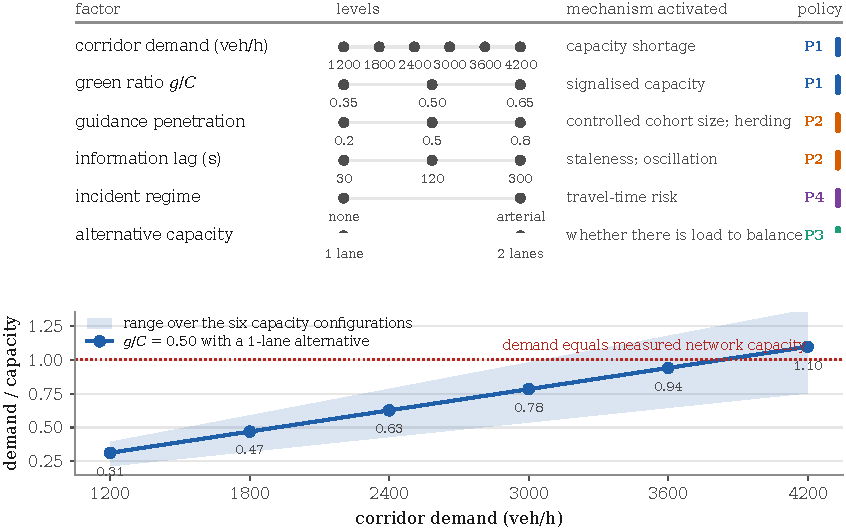
\includegraphics[width=\textwidth]{fig3_design.pdf}
\caption{Demand levels against measured network capacity. The shaded band spans
the six capacity configurations produced by the green-ratio and
alternative-capacity factors; the line marks the median configuration. The grid
spans uncongested to oversaturated conditions, and the levels follow from
measurement rather than from a chosen range.}
\label{fig:design}
\end{figure}

\subsection{Outcome Criteria and Pareto Evaluation}
\label{sec:criteria}

Three criteria (Table~\ref{tab:criteria}) capture different burdens.
\textbf{C1 mean journey time} is the travel burden per vehicle, including
insertion delay --- a policy that oversaturates the network produces vehicles
that cannot enter it, and excluding their wait would credit the policy for the
queue it caused. \textbf{C2 \CO{}} is the environmental outcome. \textbf{C3
total stopped delay} is the stationary burden, time below 0.1\,m/s in queues,
distinct from time spent travelling slowly.

All three are measured over every vehicle in the network, guided or not, with
intended departure in the measurement window, so a policy cannot be rewarded for
helping guided vehicles at the expense of background traffic. Policies are
compared by \textbf{Pareto dominance first}; the scalar cost used for regret is
C1, which requires no weights. Scalarisation appears only as sensitivity,
through three declared normalised preference profiles. No monetary value of
time, value of reliability or carbon price is used: none was available from a
verified source, and inventing one would make the conclusion an artefact of the
invented number.

\begin{table}[t]
\caption{The three decision criteria. All are measured over the same cohort:
every vehicle in the network, guided or not, whose intended departure falls in
the measurement window.}
\label{tab:criteria}
\centering\footnotesize
\begin{tabularx}{\textwidth}{@{}l l X@{}}
\toprule
& Criterion & Measurement\\
\midrule
C1 & Mean journey time (s/veh) &
  mean over the cohort of insertion delay plus in-network time. Insertion delay
  is included: a policy that oversaturates the network produces vehicles that
  cannot enter it, and excluding their wait would credit the policy for the
  queue it caused.\\[2pt]
C2 & \CO{} emissions (kg) &
  total \CO{} over the cohort, HBEFA3 passenger-car petrol Euro-4 class.\\[2pt]
C3 & Total stopped delay (veh\,s) &
  total time spent below 0.1\,m/s --- the time vehicles spend \emph{stationary}
  in queues, as distinct from the time they spend travelling slowly.\\
\bottomrule
\end{tabularx}
\end{table}

\subsection{Mechanistic Rule}

Each context is expressed through eight dimensionless descriptors computable
before activation: network saturation $x_1$; shortest-corridor saturation
$x_2 = D/\mathrm{cap}_C$; alternative capacity share $x_3$; effective green
ratio $x_4$; penetration $x_5$; information staleness
$x_6 = \Delta/T^{\mathrm{ff}}_C$; incident regime $x_7$; and controlled-flow
saturation $x_8 = p\,D/\mathrm{cap}_C$, the share of the shortest corridor's
capacity the guided cohort alone would consume. Capacities are the measured
values, so $x_1$, $x_2$ and $x_8$ are genuine degrees of saturation. A
route-overlap index is omitted: the corridors share only access and egress
edges, so overlap is structurally constant here.

The mechanistic rule B1 is an axis-aligned region rule on $x_1$--$x_8$ of depth
at most two, fitted on training contexts only. Thresholds are reported as
\emph{brackets between adjacent sampled levels}, since a grid cannot locate a
boundary more finely than its own spacing.

\subsection{Context-Aware Selector}

The learned selector predicts \emph{advantage}, not identity:
\begin{equation}
\Delta_a(x) \;=\; C(x, a_{\mathrm{SBS}}) - C(x,a),
\qquad \hat{\pi}(x) = \arg\max_a \hat{\Delta}_a(x),
\label{eq:advantage}
\end{equation}
with $a_{\mathrm{SBS}}$ determined on training contexts only. A positive
$\Delta_a$ means $a$ beats the fixed policy a deployed system would otherwise
run, so the learned quantity is the one a decision-maker needs. The model is
gradient-boosted decision trees~\cite{friedman2001gbm,ke2017lightgbm}, one
regressor per policy, with hyperparameters fixed before evaluation and never
tuned on a test fold. With a few hundred context-level instances and full
feedback from every policy, higher capacity is neither needed nor defensible; we
use no graph neural network, deep network, reinforcement learning or contextual
bandit.

The ladder is B0 fixed policy, B1 mechanistic rule, B2 depth-3 tree, B3
multinomial logistic regression, B4 the advantage selector and B5 its selective
variant, with VBS as reference. \textbf{The primary comparison is B4 against
B1}: B0 is a low bar, and beating it shows only that the decision varies with
context at all.

\subsection{Validation, Uncertainty, and Distribution Shift}

Evaluation is leave-one-context-out. Inside each fold, standardisation, the
identity of the SBS, tree thresholds, conformal quantiles and the support
envelope are recomputed from training data alone. No seed of a held-out context
appears in training, and no realised outcome is used as a feature.

\paragraph{Two gates.} B5 acts only if both pass. The \emph{support gate}
measures mean distance to the five nearest training contexts in standardised
descriptor space and abstains above the 95th percentile of the training fold's
own distances; it is a feature-space extrapolation detector. The
\emph{confidence gate} is a split-conformal interval on the predicted advantage
($\alpha=0.10$, calibrated on 30\% of the training fold); the selector acts only
when the lower bound on the advantage over the fixed policy is positive, and it
is calibrated under exchangeability, hence in-distribution. If either gate
fails, the fixed policy is used. Neither gate detects concept shift, and the
conformal guarantee does not survive covariate
shift~\cite{shimodaira2000,tibshirani2019covshift}, so we report gate behaviour
rather than coverage guarantees outside the training distribution.

\paragraph{Shift splits.} Eight held-out splits are evaluated separately and
never pooled: demand above and below the training range, an interior demand
level as an interpolation control, unseen information lag, unseen penetration,
unseen green ratio, training without disruption and testing under it, and a
disruption on a corridor that carries none in training. Pooling them would
average an interpolation control with a domain shift and hide the only thing the
experiment can say, which is that they differ.


\section{Results}

\subsection{Campaign Validity}

The main campaign executed \NumRunsMain{} runs over \NumContexts{} contexts with
\NumPolicies{} policies and \NumSeeds{} paired seeds. No run failed. Every run
completed every vehicle it generated (minimum completion \NumMinCompletion{}),
with \NumTeleports{} teleports in the entire campaign, so no result rests on a
vehicle the simulator removed. All \NumContextsAnalysed{} contexts satisfy the
validity and completeness rules declared in advance; none is excluded.

\subsection{Policy Complementarity}
\label{sec:complementarity}

The confirmatory criterion G1$'$ --- declared before the campaign and reported
here whichever way it came out --- \NumGOneVerdict{}:
\NumGOneNPolicies{} policies (\NumGOnePolicies) are strictly best in at least
one context with a seed-resolved margin. \textbf{P2 is never a resolved winner
anywhere in the factor space.} Resolved winner counts are P3 \NumWinResPThree{},
P4 \NumWinResPFour{} and P1 \NumWinResPOne{} (Table~\ref{tab:complementarity}).

The winner map is multi-factor but shallow. Naming the same policy everywhere is
correct in \NumWinMapConst{} of contexts; the best single factor
(\NumWinMapOneFactor) reaches \NumWinMapOne{}, and the best pair
\NumWinMapTwo{}. The structure is interpretable and matches the design: P1 wins
only where the shortest corridor is uncongested \emph{and} penetration is high
enough for adaptive policies to over-divert; P4 wins at low demand with generous
green; P3 wins every context at the highest demand level
(Figure~\ref{fig:regime}).

\begin{figure}[tbp]
\centering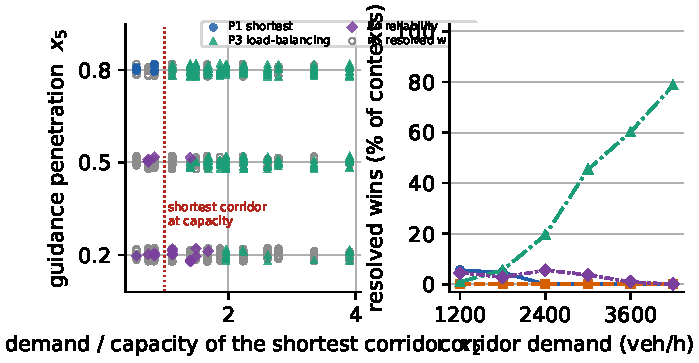
\includegraphics[width=\textwidth]{fig5_regime_map.pdf}
\caption{The regime map. Left: the resolved winner in the plane of
shortest-corridor saturation against guidance penetration; open circles mark
contexts where the seeds resolve no winner. Right: the share of contexts each
policy wins, by demand level.}
\label{fig:regime}
\end{figure}

\begin{table}[t]
\caption{Policy complementarity over 142 contexts. A win is
\emph{resolved} when the paired seed difference against the runner-up exceeds
twice its standard error. Pareto membership is over all three criteria.}
\label{tab:complementarity}
\centering\small
\begin{tabular}{@{}l r r r r@{}}
\toprule
& \multicolumn{2}{c}{Best on journey time} & \multicolumn{2}{c}{Non-dominated}\\
\cmidrule(lr){2-3}\cmidrule(lr){4-5}
& any margin & resolved & contexts & share\\
\midrule
P1 & 14 & 6 & 14 & 9.9\%\\
P2 & 42 & 0 & 74 & 52.1\%\\
P3 & 41 & 5 & 114 & 80.3\%\\
P4 & 45 & 5 & 133 & 93.7\%\\
\midrule
\multicolumn{5}{@{}l}{\emph{Pairwise differences in system mean journey time
(s/veh), positive means the first policy is slower}}\\
\midrule
Pair & mean & 5--95\% range & outcome-identical\\
\midrule
P1--P2 & +46.28 & [-1.4, +205.1] & 0.0\%\\
P1--P3 & +46.65 & [-1.6, +205.2] & 0.0\%\\
P1--P4 & +46.45 & [-1.4, +205.1] & 0.0\%\\
P2--P3 & +0.38 & [-0.5, +2.8] & 45.1\%\\
P2--P4 & +0.17 & [-0.6, +0.9] & 50.0\%\\
P3--P4 & -0.21 & [-2.4, +0.8] & 38.0\%\\
\bottomrule
\end{tabular}
\end{table}

\subsection{Decision Value of Adaptation}

Complementarity and decision value are different quantities, and here they point
in opposite directions.

The single-best fixed policy is \NumGlobalSBS{}, optimal in \NumSBSOptimalPct{}
of contexts. Figure~\ref{fig:performance} shows why: the distance-minimising policy
diverges with demand while the three adaptive policies track one another.
Running the single-best policy always costs \NumSBSMeanCost~s of system mean
journey time per vehicle; the retrospective best-per-context choice costs
\NumCostVBS~s. The headroom of Eq.~\ref{eq:headroom} is therefore
\begin{equation}
H \;=\; \NumHeadroom\ \text{s per vehicle},
\qquad
\frac{H}{\mathbb{E}_x[C(x,a_{\mathrm{SBS}})]}
\;=\; \frac{\NumHeadroom}{\NumSBSMeanCost} \;=\; \NumHeadroomPct .
\end{equation}

Selecting the wrong \emph{fixed} policy costs far more. Using the
distance-minimising policy throughout increases system mean journey time by
\NumFixedPenAbsPOne~s per vehicle relative to the single-best fixed policy, which
is \NumFixedPenPctAbsPOne{} of that policy's mean journey time of
\NumSBSMeanCost~s. The reactive and reliability-aware policies cost
\NumFixedPenPTwo~s (\NumFixedPenPctPTwo{}) and \NumFixedPenPFour~s
(\NumFixedPenPctPFour{}) on the same basis.

\begin{quote}
Choosing the fixed policy well is worth \NumFixedPenPctAbsPOne{} of mean journey
time. Choosing it \emph{per context}, given that the best fixed policy is
already in use, is worth \NumHeadroomPct{}.
\end{quote}

\subsection{Why the Adaptation Value Is Small}
\label{sec:asymmetry}

The explanation is not that the policies behave alike; Section~\ref{sec:complementarity} shows they do
not. It is that the best fixed policy is near-dominant in a measurable sense.

Define the \emph{downside} of the fixed policy as its mean loss in those
contexts where it is not best, and its \emph{upside} as its mean gain over the
best alternative in those contexts where it is. In \NumAsymNotBestPct{} of
contexts \NumGlobalSBS{} is not best, and there it loses \NumAsymLoss~s on
average (at most \NumAsymMaxLoss~s). In \NumAsymBestPct{} of contexts it is
best, and there it wins by \NumAsymMargin~s on average (at most
\NumAsymMaxMargin~s). Its upside is \textbf{\NumAsymRatio$\times$ its
downside}.

A portfolio containing such a member has a large ranking structure and a small
decision structure: any selector moving away from it risks a large loss to chase
a small gain. This is an empirical characterisation of this portfolio in this
environment, not a general theorem --- but it is measurable in any portfolio,
before a selector is built.

\begin{figure}[tbp]
\centering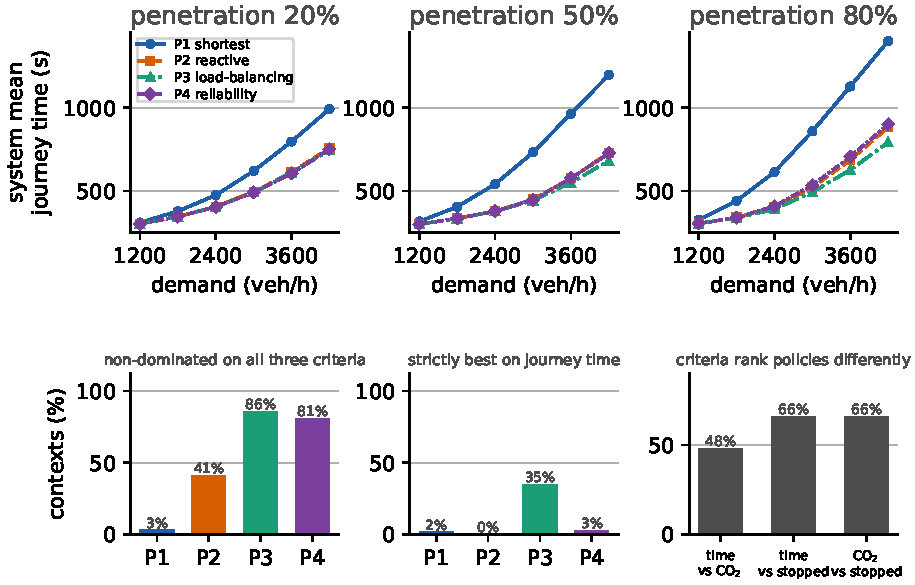
\includegraphics[width=\textwidth]{fig4_performance_pareto.pdf}
\caption{System mean journey time against demand at each guidance penetration
level, averaged over the remaining factors. The distance-minimising policy
diverges once the shortest corridor saturates, while the three adaptive policies
track one another closely --- the visual form of the small decision value
quantified in Section~\ref{sec:asymmetry}.}
\label{fig:performance}
\end{figure}

\subsection{Noise and Resolution of the Adaptation Effect}

Among the \NumResolvNContexts{} contexts where the fixed policy is not best, the
mean headroom is \NumResolvHeadroomNZ~s against a mean two-standard-error band
of \NumResolvNoiseNZ~s on the same paired comparison, and the headroom exceeds
its own noise in \NumResolvExceeds{} of them (\NumResolvExceedsPct{}). Resolving
the campaign-wide mean effect of \NumResolvHeadroom~s would require roughly
\NumResolvSeedsNeeded{} seeds per context, about \NumResolvRunsNeeded{} runs.
We report this rather than presenting a near-noise-floor improvement as an
achievement.

\subsection{Mechanistic Rule}

Fitted on all contexts for exposition, the depth-2 rule splits first on
$\NumMechFeature = p\,D/\mathrm{cap}_C$, the share of the shortest corridor's
capacity the guided cohort alone would consume, at a threshold bracketed between
\NumMechBracketLo{} and \NumMechBracketHi{}. The rule is physically readable:
below that share the decision turns on the effective green ratio; above it, on
whether the arterial is already oversaturated (Figure~\ref{fig:regions}).

The rule identifies the best policy in \NumMechTopOne{} of contexts, more often
than always naming the fixed policy. Its mean decision regret is nevertheless
\NumMechRegret~s against \NumMechFixedRegret~s for the fixed policy.
\textbf{It is more accurate and more costly.} Under leave-one-context-out the
same pattern holds: B1 reaches \NumBOneTopOne{} top-1 accuracy against B0's
\NumBZeroTopOne{}, and \NumBOneRegret~s of regret against \NumBZeroRegret~s.

This is the predict-then-optimise distinction~\cite{elmachtoub2022spo} in a
traffic setting. A rule trained to name the winner is rewarded for being right
where the margin is negligible and punished only mildly for being wrong where it
is large --- the wrong trade under an \NumAsymRatio$\times$ asymmetry.

\begin{figure}[tbp]
\centering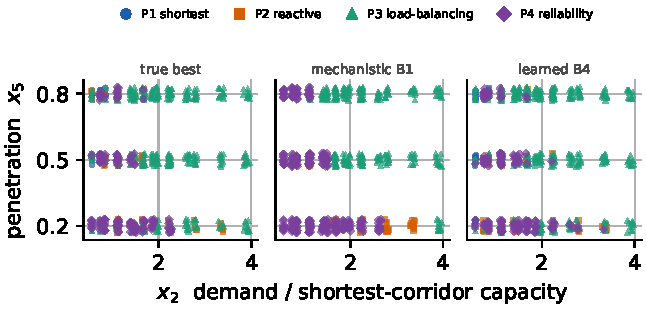
\includegraphics[width=\textwidth]{fig6_selection_regions.pdf}
\caption{Selection regions in the mechanistic feature space: the true best
policy, the depth-2 mechanistic rule, and the advantage-based selector, over
controlled-flow saturation and guidance penetration.}
\label{fig:regions}
\end{figure}

\subsection{Advantage-Based Selector}

Predicting advantage (Eq.~\ref{eq:advantage}) rather than identity reverses the
failure. B4 reaches \NumBFourRegret~s of mean regret, closing
\NumBFourGapClosed{} of the gap between the fixed policy and the retrospective
best, while being \emph{less} accurate at naming the winner (\NumBFourTopOne{})
than the logistic baseline (\NumBThreeTopOne{}, \NumBThreeRegret~s). It also has
the lowest maximum regret of any selector, \NumBFourMax~s against
\NumBZeroMax~s (Table~\ref{tab:ladder}, Figure~\ref{fig:ladder}).

The primary comparison declared in advance was B4 against B1, and B4 wins it
decisively: \NumBFourRegret~s against \NumBOneRegret~s. Beating B0 alone would
not have been evidence of much, since B0 is near-dominant by
Section~\ref{sec:asymmetry}.

The magnitude is what matters operationally. B4 reduces mean regret by
\NumBFourVsBZero~s per vehicle relative to the fixed policy --- 
\NumBFourVsBZeroPct{} of a \NumSBSMeanCost~s mean journey time. The selector is
real and reproducible, and below the threshold at which an operator would act on
it.

\begin{table}[t]
\caption{Decision quality under leave-one-context-out evaluation. Regret is in
seconds of system mean journey time per vehicle. ``Within noise'' is the share
of contexts whose regret falls below that context's own seed noise floor.}
\label{tab:ladder}
\centering\small
\begin{tabular}{@{}l r r r r r r@{}}
\toprule
& \multicolumn{4}{c}{Decision regret (s/veh)} & within & gap closed\\
\cmidrule(lr){2-5}
& mean & median & max & CVaR$_{90}$ & noise & vs.\ SBS\\
\midrule
B0 ~~best fixed policy (SBS) & 0.45 & 0.00 & 17.2 & 3.7 & 99\% & ---\\
B1 ~~mechanistic rule & 0.77 & 0.00 & 17.2 & 6.5 & 96\% & -0.714\\
B2 ~~decision tree, depth 3 & 0.34 & 0.00 & 17.2 & 3.0 & 99\% & 0.238\\
B3 ~~multinomial logistic & 0.28 & 0.00 & 17.2 & 2.5 & 100\% & 0.373\\
B4 ~~GBDT advantage selector & 0.20 & 0.00 & 7.0 & 1.7 & 100\% & 0.558\\
B5 ~~selective GBDT with abstention & 0.45 & 0.00 & 17.2 & 3.7 & 99\% & 0.000\\
~~~~~~VBS (retrospective, not deployable) & 0.00 & 0.00 & 0.0 & 0.0 & 100\% & 1.000\\
\bottomrule
\end{tabular}
\end{table}

\begin{figure}[tbp]
\centering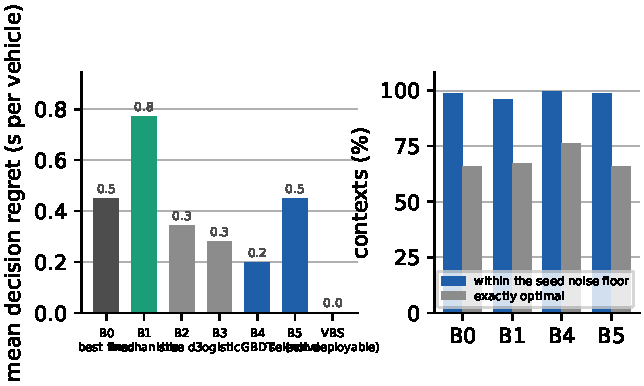
\includegraphics[width=\textwidth]{fig7_decision_ladder.pdf}
\caption{Decision quality under leave-one-context-out evaluation. Left: mean
regret for each selector; the retrospective best is hatched because it is not
deployable. Right: the share of contexts in which each selector is within the
seed noise floor, and exactly optimal.}
\label{fig:ladder}
\end{figure}

\subsection{Selective Prediction and Distribution Shift}

B5 abstains in \NumAbstainRate{} of in-distribution contexts and returns exactly
the fixed policy's regret, \NumBFiveRegret~s. The mechanism is explicit: the
conformal interval on the predicted advantage is wider than the advantage, so
the requirement that its lower bound exceed zero is never met. A calibrated gate
refuses to act on an effect smaller than its own uncertainty.

Across the \NumOODNTotal{} shift splits (Table~\ref{tab:ood},
Figure~\ref{fig:ood}), the unguarded selector B4 does not behave uniformly. Using
a tolerance of \NumOODTolerance~s per vehicle, it \textbf{helps} on
\NumOODNHelps{} splits, is \textbf{indistinguishable} on \NumOODNNeutral{}, and
\textbf{harms} on \NumOODNHarms{}:
\begin{itemize}
\item \emph{helps}: the interpolation control O3 (\NumOODThreeMidBZero{} to
\NumOODThreeMidBFour~s) and, notably, the domain shift O8
(\NumOODEightNorthBZero{} to \NumOODEightNorthBFour~s);
\item \emph{indistinguishable}: unseen low demand O2, unseen lag O4, unseen
penetration O5;
\item \emph{harms}: unseen high demand O1 (\NumOODOneHighBZero{} to
\NumOODOneHighBFour~s), unseen green ratio O6, and worst of all the concept
shift O7 (\NumOODSevenIncBZero{} to \NumOODSevenIncBFour~s).
\end{itemize}
\textbf{On every one of the \NumOODNHarms{} harmful splits, B5 recovered the
fixed policy's regret exactly.} The selective rule therefore prevented the
observed harms; it does not guarantee protection against harms not observed
here.

The support gate flags \NumOODFourLagSupport{}, \NumOODFivePenSupport{} and
\NumOODSixGreenSupport{} of held-out contexts as outside the training envelope
on the lag, penetration and green-ratio extrapolations respectively. B1 degrades
worst of all under shift, reaching \NumOODFivePenBOne~s on unseen penetration.

\paragraph{A shift the gate cannot see.} O8 is instructive precisely because the
support gate does \emph{not} fire: it flags \NumOODEightNorthSupport{} of
held-out contexts, because those contexts' descriptors are identical to
descriptors seen in training --- the incident's \emph{location} is not among the
eight. The selector happens to do well there, but it does so unguarded. A
support gate defined on a feature space cannot detect a shift that leaves that
feature space unchanged, and this is a concrete instance rather than a
theoretical caveat.

\begin{table}[t]
\caption{Distribution shift, reported separately by shift type. Regret in
seconds of system mean journey time per vehicle on the held-out regime. The
support column is the share of held-out contexts the support gate flagged as
outside the training envelope.}
\label{tab:ood}
\centering\small
\begin{tabular}{@{}l l l r r r r r r@{}}
\toprule
& Held out & Shift type & B0 & B1 & B4 & B5 & flagged & abstained\\
\midrule
O2 & demand = 1200.0 & extrapolation & 0.53 & 0.63 & 0.53 & 0.53 & 100\% & 0\%\\
O4 & lag = 300.0 & extrapolation & 0.49 & 0.42 & 0.69 & 0.49 & 100\% & 63\%\\
O5 & penetration = 0.8 & extrapolation & 1.56 & 1.01 & 0.38 & 1.56 & 100\% & 54\%\\
O6 & gc = 0.65 & extrapolation & 0.95 & 1.67 & 0.68 & 0.95 & 100\% & 86\%\\
O7 & incident = 1.0 & covariate + concept shift & 0.21 & 1.62 & 5.57 & 0.21 & 0\% & 64\%\\
\bottomrule
\end{tabular}
\end{table}

\begin{figure}[tbp]
\centering
\includegraphics[width=\textwidth]{fig8_ood.pdf}
\caption{Distribution shift, reported separately by shift type. Top: mean regret
on the held-out regime for each selector. Bottom: the share of held-out contexts
flagged outside the training support, and the share on which the selective
selector abstained.}
\label{fig:ood}
\end{figure}

\subsection{Boundary Refinement}
\label{sec:boundary}

Where the main grid showed the preferred policy changing between adjacent demand
levels, three intermediate levels were run in each of the \NumBoundN{}
widest-margin cells.

\NumBoundMono{} of \NumBoundN{} refined sequences are monotone, with a single
change point, and in point estimate they narrow the switching bracket from the
\NumBoundGrid~veh/h grid spacing to a median of \NumBoundWidth~veh/h. All
\NumBoundPOneN{} shortest-to-load-balancing transitions are monotone; their
change points sit in a \NumBoundWidth~veh/h bracket whose position differs by
cell, from \NumBoundPOneEarliestLo--\NumBoundPOneEarliestHi~veh/h to
\NumBoundPOneLatestLo--\NumBoundPOneLatestHi~veh/h. That the position moves with
the cell is the point: the boundary is a property of the operating conditions,
not a single number for the network.

\textbf{None of these refined steps is seed-resolved.} The point estimates move
consistently, but no individual step between adjacent refined levels exceeds
twice its own standard error at \NumSeeds{} seeds. The remaining
\NumBoundNonMono{} sequences are non-monotone, and all involve the
reliability-aware policy. We therefore report the transition as a point-estimate
bracket and state that it is unresolved: the shortest-path to load-balancing
reversal is an ordered regime change, while the apparent reliability-aware
transitions near it are not distinguishable from noise.

\subsection{Three-Criterion Pareto Structure}
\label{sec:pareto}

Over all \NumContextsAnalysed{} contexts, \NumParetoNonSingleton{} have a
non-singleton Pareto set. Non-domination is not concentrated in one policy: P3
is non-dominated in \NumParetoPctPThree{} of contexts, P4 in
\NumParetoPctPFour{}, P2 in \NumParetoPctPTwo{} and P1 in \NumParetoPctPOne{}.

The criteria are not interchangeable. Journey time and \CO{} correlate at
\NumCorrCOneCTwo{} and rank the four policies identically in
\NumSameOrderCOneCTwo{} of contexts; journey time and stopped delay correlate at
\NumCorrCOneCThree{} and agree in only \NumSameOrderCOneCThree{}. The best
policy on \CO{} differs from the best on journey time in
\NumBestCTwoDiffersPct{} of contexts; on stopped delay it differs in
\NumBestCThreeDiffersPct{}.

The policies specialise by criterion rather than by regime.
\NumSpecCOnePolicy{} minimises journey time in \NumSpecCOneN{} contexts and
\NumSpecCTwoPolicy{} minimises \CO{} in \NumSpecCTwoN{}, but
\textbf{\NumSpecCThreePolicy{} minimises stopped delay in \NumSpecCThreeN{}
contexts (\NumSpecCThreePct{})} while minimising journey time in only
\NumSpecCOnePFour{}. The reliability-aware policy routes towards the steady,
unsignalised corridor: its vehicles spend less time stationary and more time
moving. \textbf{This is where the portfolio's complementarity lives} --- on the
criterion vector, not on the scalar cost.

\paragraph{Eco-routing remains excluded, on evidence.} \CO{} and journey time
correlate at \NumCorrCOneCTwo{} and select the same policy in
\NumSameOrderCOneCTwo{} of contexts. An objective nearly monotone in travel time
adds a label rather than a policy; the numbers are given so a reader may
disagree with the threshold rather than with an assertion.

\begin{table}[t]
\caption{Sensitivity and robustness. Upper: the two policy parameters frozen
before the experiment, the effect of changing each on that policy's own mean
journey time, and how often the identity of the best policy is unchanged.
Lower: the three declared preference profiles over normalised criteria, the
policy each selects, and how often that agrees with the journey-time choice.}
\label{tab:sensitivity}
\centering\footnotesize
\setlength{\tabcolsep}{4pt}
\begin{tabular}{@{}l l r r r r r@{}}
\toprule
\multicolumn{7}{@{}l}{\emph{Policy parameters}}\\
\midrule
Policy & Param. & Frozen & Alt. & $\Delta$ (s) & $\Delta$ (\%) & winner same\\
\midrule
P3 & \texttt{p3\_eps} & 0.2 & 0.1 & +8.10 & +1.27\% & 84\%\\
P3 & \texttt{p3\_eps} & 0.2 & 0.3 & -16.66 & -2.62\% & 78\%\\
P4 & \texttt{p4\_lambda} & 1.0 & 0.5 & -0.11 & +0.00\% & 91\%\\
P4 & \texttt{p4\_lambda} & 1.0 & 1.5 & +1.27 & +0.16\% & 98\%\\
\midrule
\multicolumn{7}{@{}l}{\emph{Preference profiles} (weights on normalised C1--C3)}\\
\midrule
Profile & Weights & P1 & P2 & P3 & P4 & agrees C1\\
\midrule
Time & (0.70, 0.15, 0.15) & 19 & 76 & 406 & 147 & 92.9\%\\
Balanced & (0.40, 0.30, 0.30) & 8 & 70 & 399 & 171 & 86.0\%\\
Environment & (0.20, 0.55, 0.25) & 7 & 66 & 425 & 150 & 80.1\%\\
\bottomrule
\end{tabular}
\end{table}

\subsection{Sensitivity}
\label{sec:sensitivity}

Across the three declared preference profiles the preferred policy changes in
\NumPrefChanges{} of contexts (Table~\ref{tab:sensitivity}). The journey-time
choice is reproduced by the time-weighted profile in \NumPrefAgreeTime{} of
contexts, the balanced profile in \NumPrefAgreeBalanced{} and the
environment-weighted profile in \NumPrefAgreeEnvironment{}. The decision is
stable under reasonable preference assumptions, and where it is not, stopped
delay is what moves it.

The two frozen policy parameters behave differently. The dispersion weight of
the reliability-aware policy is close to immaterial, changing that policy's own
mean journey time by at most \NumLambdaMaxChangePct{}; across all four parameter
changes the identity of the best policy is unchanged in \NumWinnerStableMin{} to
\NumWinnerStableMax{} of the contexts tested. The admissibility tolerance of the
load-balancing policy is not immaterial: loosening it from \NumEpsFrozen{} to
\NumEpsAlt{} improves that policy's own mean journey time by \NumEpsGainPct{}
(\NumEpsGainSec~s). The frozen value therefore \emph{understates} how dominant
the load-balancing policy is, which strengthens rather than weakens the central
conclusion. We report this rather than retrofitting the better value.


\section{Experimental Integrity and Deviations}
\label{sec:integrity}

\paragraph{What was frozen, and when.} The experiment specification --- factors
and levels, criteria, seed count, the resolution criterion, screening gates,
baseline ladder, model class and hyperparameters, abstention rules and shift
splits --- was written and committed to version control \emph{before any
evaluation run was executed}. Policy parameters were frozen at the same time and
varied afterwards only as sensitivity (Section~\ref{sec:sensitivity}). No factor level was chosen
because it produced a particular outcome; the demand levels follow from measured
capacity.

\paragraph{Execution reconciliation.} The main campaign comprises
\NumRunsMain{} valid runs ($\NumContexts \times \NumPolicies \times \NumSeeds$),
and this is the number underlying every result in Section~5 unless stated
otherwise. The project executed \NumRunsTotalAttempted{} simulations in total,
of which \NumRunsTotalSucceeded{} succeeded: \NumRunsValidate{}
scenario-validation, \NumRunsScreen{} screening, \NumRunsMain{} main,
\NumRunsSens{} sensitivity, \NumRunsOODNorth{} domain-shift and
\NumRunsBoundary{} boundary-refinement runs, plus \NumRunsFailedBypass{} runs
that failed for the reason given below. These counts are distinct and are not
interchangeable.

\paragraph{Protocol deviation D-1.} The pre-specified complementarity screen did
not satisfy criterion G1 and therefore triggered the declared stopping rule. The
main campaign was nevertheless executed, under the documented protocol deviation
D-1. The reasons for continuation were recorded before campaign launch: a
selection problem demonstrably existed; G1 was written against the scalar
criterion and was blind to the three-criterion structure beside it; and the
negative finding rested on 16 of \NumContexts{} contexts sampled at extreme
factor levels only. A confirmatory criterion G1$'$, declared before the main
campaign and identical in definition to G1, was then evaluated on all
\NumContexts{} contexts. G1$'$ \NumGOneVerdict{}
(Section~\ref{sec:complementarity}).

We do not present G1$'$ as erasing the deviation, and we do not describe the
original screen as having passed. It did not. The methodological lesson is that
the screen sampled corner conditions and did not sample the interior transition
region, so it had power to detect near-ties but not coverage to find where the
minority policies win. A resolution-IV fraction at extreme levels is an
efficient design for main effects and a poor one for discovering where a winner
map changes. That is a limitation of our screening design, not a justification
for having continued.

\paragraph{An infeasible shift split and its replacement.} One declared shift
split placed the disruption on the bypass corridor. The bypass is single-lane,
so the specified capacity-reducing lane closure does not constrain it --- it
disconnects it, leaving vehicles already routed there without a valid path. All
\NumRunsFailedBypass{} attempted runs failed for this reason. The split was
replaced by the nearest feasible construction, a disruption on the two-lane
north corridor, which preserves the intent (a corridor carrying no disruption in
any training context) while remaining a capacity reduction rather than a
severance. A guard now refuses any incident on a single-lane edge. The
replacement is reported as split O8 and is \emph{not} the originally declared
split.

\paragraph{Traceability.} Every numeric claim in this paper is generated from a
single machine-readable results file by a script, and rendered through a macro;
a build-time check fails if the text references a quantity the analysis did not
produce. Seventeen automated quality-control checks cover leakage discipline,
training-fold-only baseline selection, freeze ordering, shift reporting and
citation completeness. All \NumRefs{} references were verified against publisher
records; DOIs that could not be confirmed directly were omitted rather than
inferred.

\section{Discussion}

\subsection{Complementarity Does Not Imply Adaptation Value}

The portfolio is complementary: three policies win somewhere by a resolved
margin, the winner map needs more than one factor, and
\NumParetoNonSingleton{} of contexts have a non-singleton Pareto set. On the
usual reading, that is the evidence for building a selector.

It is not sufficient evidence. The decision value of the entire winner map is
\NumHeadroom~s per vehicle, \NumHeadroomPct{} of the mean journey time under the
single-best fixed policy, because that policy's upside where it wins is
\NumAsymRatio$\times$ its downside where it does not. The two quantities are
computable from the same data, one is small when the other is large, and only
the second determines whether adaptation is worth attempting.

The practical implication is a cheap first step. Before choosing a model class,
compute the gap between the best fixed policy and the retrospective best, and
compare it with the noise floor of that same paired comparison. Neither requires
a model. Had we done so here, the answer would have been a \NumHeadroomPct{} gap
sitting close to the resolution of a \NumSeeds{}-seed design.

\subsection{Decision-Oriented Evaluation Changes the Interpretation of Accuracy}

Selection accuracy and decision regret rank the methods differently in this
study, and the disagreement is not marginal. The mechanistic rule is more
accurate than the fixed policy (\NumBOneTopOne{} versus \NumBZeroTopOne{}) and
more costly (\NumBOneRegret~s versus \NumBZeroRegret~s). The advantage-based
selector is less accurate than the logistic baseline and cheaper than it.

The cause is not model capacity but the training target. Methods trained to name
the winner optimise a loss that treats every context alike; a context where the
margin is 20\,s contributes no more than one where it is 0.2\,s. Predicting
advantage weights each context by what is actually at stake, which under an
\NumAsymRatio$\times$ asymmetry is the difference between a selector that helps
and one that hurts. This is the predict-then-optimise
argument~\cite{elmachtoub2022spo}, appearing here not as a refinement but as a
sign change.

For anyone reporting such a system: report decision regret, and do not present
selection accuracy as a proxy for it.

\subsection{A Strong Fixed Policy Can Be a Rational Default}

In this benchmark the load-balancing policy is optimal in
\NumSBSOptimalPct{} of contexts and loses only \NumAsymLoss~s on average where
it is not. Against that, the distance-minimising policy costs
\NumFixedPenAbsPOne~s per vehicle more --- \NumFixedPenPctAbsPOne{} of the
single-best policy's \NumSBSMeanCost~s mean journey time.

Two decisions therefore sit three orders of magnitude apart: which fixed policy
to run, and whether to vary it by context. A benchmark that reports only the
second makes the first invisible.

\subsection{Selective Adaptation and the Limits of Feature-Space Support}

The selective rule prevented the observed harms: on each of the
\NumOODNHarms{} harmful shift splits it recovered the fixed policy's regret
exactly. It did so by declining to act --- the conformal interval is wider than
the effect --- and the price is the in-distribution gain the unguarded selector
achieves.

Its limits are equally concrete. The conformal gate is calibrated under
exchangeability and so is an in-distribution instrument; the support gate is a
feature-space extrapolation detector; neither detects concept shift. Split O8
shows what that means in practice: a disruption moved to a corridor carrying
none in training left every descriptor unchanged, the support gate flagged
\NumOODEightNorthSupport{} of those contexts, and the selector acted unguarded.
It happened to do well. A support gate cannot detect a shift its feature space
does not represent, and reporting the case is more useful than asserting the
principle.

\subsection{Implications for Routing-Policy Deployment}

We state what this benchmark demonstrates, not what an operator should do.

The benchmark shows that in this environment the decision carrying the
substantial value is the choice of fixed policy, and that the incremental value
of context-dependent selection is small relative to it and close to the
resolution of the experiment. It shows that if such a selector is built, the
training target determines whether it helps, and that a support-and-confidence
gate removed the harms observed under shift while also removing the gains. And
it shows that the criterion matters as much as the policy: the policy
minimising stopped delay is not the policy minimising journey time in
\NumBestCThreeDiffersPct{} of contexts, which is a different argmin rather than
a preference weighting.

Whether these carry to a real network is not established by anything here.

\section{Limitations}

\paragraph{Environment and scope.} The network is synthetic: a controlled
instrument built to isolate mechanisms, not a model of any city. Corridor demand
is a single origin--destination pair choosing among three corridors; the four
minor streets couple the routing decision to traffic that is not routed, but
many simultaneously-routed pairs, with the interactions between their choices,
are outside what is tested. No claim of real-world validation is made anywhere
in this paper. What is portable is the method rather than the numbers: the
descriptors are dimensionless, so a boundary is stated as a degree of saturation
and a controlled-flow share, both measurable on a real network.

\paragraph{Decision context and compliance.} The selector is given the operating
conditions; a deployed system would have to forecast them and would inherit the
forecast's error on top of the selector's. Guided vehicles comply fully with the
policy, and unguided vehicles never respond to conditions at all; real behaviour
lies between these. The reported decision quality is therefore an upper bound on
what the same selector would achieve behind a forecast and partial compliance.

\paragraph{Resolution and statistical reach.} The experiment samples a finite
grid with \NumSeeds{} seeds. Boundaries are reported as brackets between
adjacent sampled levels and never as continuous thresholds, and no refined
switching step is seed-resolved (Section~5.9); resolving the campaign-wide
adaptation effect would need roughly \NumResolvSeedsNeeded{} seeds per context.
Where a factor is associated with a change of preferred policy, that is an
association within a designed factorial, not an identified causal mechanism.

\paragraph{Protocol.} Two deviations are on the record and are described in
Section~\ref{sec:integrity}: the screening gate G1 failed and the campaign proceeded under
deviation D-1, and one declared shift split was infeasible and was replaced by
the nearest feasible construction. Neither is presented as neutral.

\paragraph{Uncertainty machinery.} Split conformal coverage requires
exchangeability, which covariate shift breaks; the conformal gate is calibrated
in-distribution and heuristic outside it, the support gate detects only
extrapolation visible in the feature space, and neither detects concept shift.
Split O8 is a demonstrated instance of a shift the support gate does not see.

\paragraph{Frozen parameters and the emission model.} The policy parameters were
fixed before the experiment and are not optima; a better-tuned load-balancing
tolerance improves that policy by \NumEpsGainPct{}, which strengthens the
central conclusion but means the reported value is not the best available.
\CO{} is computed by the simulator's HBEFA3 implementation for one vehicle
class, without fleet composition, cold starts or gradient, so C2 should be read
as a consistent comparative index rather than an absolute emissions estimate.
Finally, no monetary valuation is used anywhere, which keeps the study free of
invented constants but also means it cannot express a trade-off in currency.

\section{Conclusion}

We characterised context-dependent selection among four established urban
routing policies in \NumRunsMain{} microsimulation runs over \NumContexts{}
controlled contexts, with every policy decision taken from information available
before activation and every comparison paired under common random numbers.

The portfolio is complementary: three of four policies are strictly best
somewhere by a seed-resolved margin, the winner map depends on more than one
factor, and \NumParetoNonSingleton{} of contexts have a non-singleton Pareto set
over journey time, \CO{} and stopped delay. The reliability-aware policy, which
rarely minimises journey time, minimises stopped delay in \NumSpecCThreePct{} of
contexts. Complementarity in this portfolio lives in the criterion vector rather
than in the scalar cost.

Exploiting it is nevertheless worth \NumHeadroom~s of system mean journey time
per vehicle, \NumHeadroomPct{} of the single-best fixed policy's
\NumSBSMeanCost~s, because that policy's upside where it wins is
\NumAsymRatio$\times$ its downside where it does not. Selecting the wrong fixed
policy costs \NumFixedPenAbsPOne~s per vehicle, \NumFixedPenPctAbsPOne{} of the
same baseline.

Within that margin the methodological findings are clear. A selector trained to
predict the winner's identity is more accurate than the fixed policy and more
costly than it; one trained to predict each policy's advantage is less accurate
and closes \NumBFourGapClosed{} of the available gap. Across
\NumOODNTotal{} shift splits the unguarded selector helped on \NumOODNHelps{},
was indistinguishable on \NumOODNNeutral{} and harmed on \NumOODNHarms{}, and a
support-and-confidence gate recovered the fixed policy exactly on every harmful
split while forgoing the in-distribution gain. One split showed a shift the
support gate cannot see, because it left the feature space unchanged.

The benchmark's contribution is to separate three questions usually treated as
one: whether policies are complementary, whether adaptation carries decision
value, and whether a selector can be deployed safely. Here the answers are yes,
barely, and only with a gate that mostly declines to act. Both of the first two
quantities are measurable before any model is built, and we suggest measuring
them first.


\section*{Reproducibility}
All scenario, policy, simulation and analysis code, every run record, and the
scripts generating every number, table and figure are provided with the
submission. The experiment specification was committed before any evaluation run
was executed; both protocol deviations are documented in
Section~\ref{sec:integrity}.

\bibliographystyle{splncs04}
\bibliography{references}

\end{document}
